\documentclass[12pt]{amsart}
\usepackage{amsmath,latexsym,amssymb}
\usepackage{tikz}
\usetikzlibrary{arrows,automata}

\begin{document}

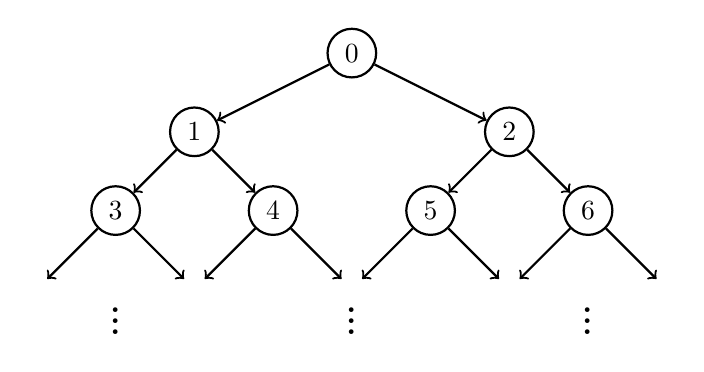
\begin{tikzpicture}[thick] 
\node[draw,circle] (0) at (4,4) {$0$};
\node[draw,circle] (1) at (2,3) {$1$};
\node[draw,circle] (2) at (6,3) {$2$};
\node[draw,circle] (3) at (1,2) {$3$};
\node[draw,circle] (4) at (3,2) {$4$};
\node[draw,circle] (5) at (5,2) {$5$};
\node[draw,circle] (6) at (7,2) {$6$};
\node (7) at (0,1) {};
\node (8) at (2,1) {};
\node (9) at (4,1) {};
\node (10) at (6,1) {};
\node (11) at (8,1) {};
\node (12) at (1,0.7) {\huge{$\vdots$}};
\node (13) at (4,0.7) {\huge{$\vdots$}};
\node (14) at (7,0.7) {\huge{$\vdots$}};
\draw[->] (0)--(1);
\draw[->] (0)--(2);
\draw[->] (1)--(3);
\draw[->] (1)--(4);
\draw[->] (2)--(5);
\draw[->] (2)--(6);
\draw[->] (3)--(7);
\draw[->] (3)--(8);
\draw[->] (4)--(8);
\draw[->] (4)--(9);
\draw[->] (5)--(9);
\draw[->] (5)--(10);
\draw[->] (6)--(10);
\draw[->] (6)--(11);
\end{tikzpicture}

\end{document}